\begin{frame}
\frametitle{Geometric morphometrics}
\begin{quote}
``We are now in the midst of a {\bf revolution in morphometric methodology}. The new approaches are more effective in capturing information about the shape of an organism and result in {\bf more powerful statistical procedures} for testing for differences in shape. They are also {\bf more effective in enabling a researcher to visualize differences} in shape and in suggesting simple traditional measurements that could be used in future studies.''
\end{quote}

\vspace{0.25cm}

\begin{tiny}
FJ Rohlf \& LF Marcus. ``A Revolution in Morphometrics''. Trends in Ecology \& Evolution 8.4: 129-132 (1993).\par
\end{tiny}
\end{frame}

\begin{frame}
\frametitle{D'Arcy Thompson's approach}
\begin{quote}
``...diverse and dissimilar fishes can be referred as a whole to identical functions of very different co-ordinate systems...''
\end{quote}
\begin{center}
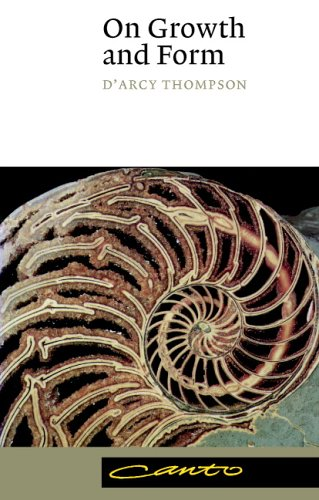
\includegraphics[height=0.4\textheight]{OGAF}
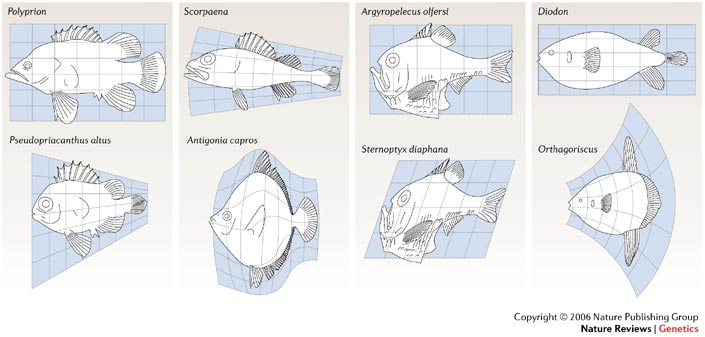
\includegraphics[height=0.4\textheight]{fish}
\end{center}
We can compute relative shapes using image registration.
\end{frame}



\begin{frame}
\frametitle{Geometric morphometrics}
\begin{enumerate}
\item Data are recorded to capture the geometry in the form of 2D or 3D {\bf coordinates of landmark points}.
\item Geometric relationships among landmarks are not inherent in the raw coordinates themselves.  {\bf The relationship among points is captured by fitting an appropriate function to them} in 2 or 3D.
\item {\bf The analyses are designed to indicate directions of maximum variation} and hence may suggest which conventional variables one should emphasize in verbal descriptions of the results.
\item Displays of the results of the analyses are emphasized, using {\bf differences or changes that can be shown on pictorial representations} of the organisms studied.  
\end{enumerate}

\vspace{0.25cm}

\begin{tiny}
Plagiarised from FJ Rohlf \& LF Marcus. ``A Revolution in Morphometrics''. Trends in Ecology \& Evolution 8.4: 129-132 (1993).\par
\end{tiny}
\end{frame}



\begin{frame}
\frametitle{Geometric morphometrics}
Classic multivariate statistical methods used:
\begin{itemize}
\item Procrustes analysis
\item Principal Component Analysis (PCA)
\item Canonical Correlation Analysis (CCA)
\item Multivariate ANalysis of COVAriance (MANCOVA)
\item Discriminant functions
\end{itemize}
These appraches could be augmented by pattern recognition and other machine learning techniques.
\end{frame}



\begin{frame}
\frametitle{Encoding geometry}
\begin{columns}[c]
\column{0.55\textwidth}
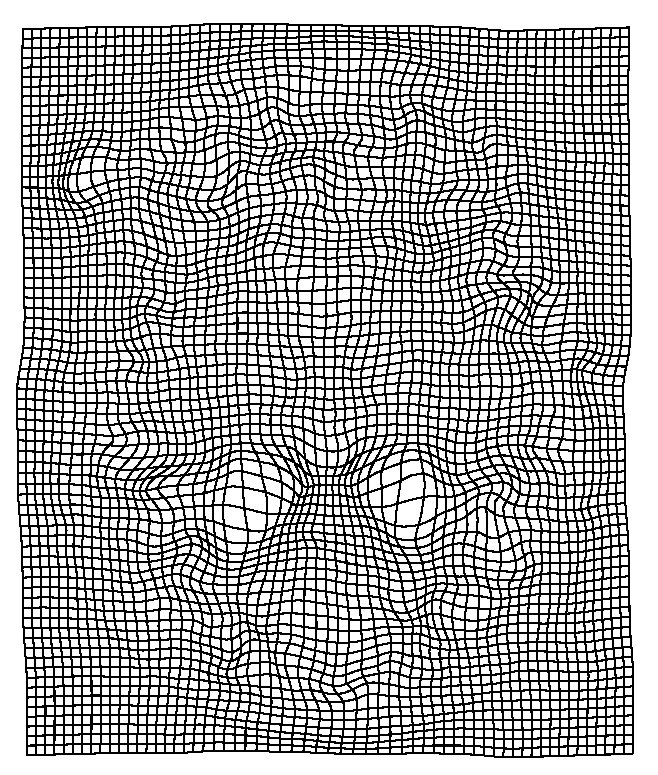
\includegraphics[width=\textwidth]{def}
\column{0.45\textwidth}
\begin{itemize}
\item Manual definition of landmarks is laborious, subjective and not very reproducible.
\item Relatively few landmarks in the brain.
\item Image registration is easier.
\item Can apply the tools of geometric morphometrics (statistical shape analysis) to automatically estimated deformations.
\end{itemize}
\end{columns}
\end{frame}

